\documentclass[9pt]{article}\usepackage[]{graphicx}\usepackage[]{xcolor}
% maxwidth is the original width if it is less than linewidth
% otherwise use linewidth (to make sure the graphics do not exceed the margin)
\makeatletter
\def\maxwidth{ %
  \ifdim\Gin@nat@width>\linewidth
    \linewidth
  \else
    \Gin@nat@width
  \fi
}
\makeatother

\definecolor{fgcolor}{rgb}{0.345, 0.345, 0.345}
\newcommand{\hlnum}[1]{\textcolor[rgb]{0.686,0.059,0.569}{#1}}%
\newcommand{\hlstr}[1]{\textcolor[rgb]{0.192,0.494,0.8}{#1}}%
\newcommand{\hlcom}[1]{\textcolor[rgb]{0.678,0.584,0.686}{\textit{#1}}}%
\newcommand{\hlopt}[1]{\textcolor[rgb]{0,0,0}{#1}}%
\newcommand{\hlstd}[1]{\textcolor[rgb]{0.345,0.345,0.345}{#1}}%
\newcommand{\hlkwa}[1]{\textcolor[rgb]{0.161,0.373,0.58}{\textbf{#1}}}%
\newcommand{\hlkwb}[1]{\textcolor[rgb]{0.69,0.353,0.396}{#1}}%
\newcommand{\hlkwc}[1]{\textcolor[rgb]{0.333,0.667,0.333}{#1}}%
\newcommand{\hlkwd}[1]{\textcolor[rgb]{0.737,0.353,0.396}{\textbf{#1}}}%
\let\hlipl\hlkwb

\usepackage{framed}
\makeatletter
\newenvironment{kframe}{%
 \def\at@end@of@kframe{}%
 \ifinner\ifhmode%
  \def\at@end@of@kframe{\end{minipage}}%
  \begin{minipage}{\columnwidth}%
 \fi\fi%
 \def\FrameCommand##1{\hskip\@totalleftmargin \hskip-\fboxsep
 \colorbox{shadecolor}{##1}\hskip-\fboxsep
     % There is no \\@totalrightmargin, so:
     \hskip-\linewidth \hskip-\@totalleftmargin \hskip\columnwidth}%
 \MakeFramed {\advance\hsize-\width
   \@totalleftmargin\z@ \linewidth\hsize
   \@setminipage}}%
 {\par\unskip\endMakeFramed%
 \at@end@of@kframe}
\makeatother

\definecolor{shadecolor}{rgb}{.97, .97, .97}
\definecolor{messagecolor}{rgb}{0, 0, 0}
\definecolor{warningcolor}{rgb}{1, 0, 1}
\definecolor{errorcolor}{rgb}{1, 0, 0}
\newenvironment{knitrout}{}{} % an empty environment to be redefined in TeX

\usepackage{alltt}
\usepackage{multicol}
\usepackage{amssymb,mathrsfs,graphicx}
\usepackage{enumerate}
\usepackage{amsthm}
\usepackage{lscape}
\usepackage{pdfpages}
\theoremstyle{definition}
\newtheorem{definition}{Definition}[section]

\theoremstyle{remark}
\newtheorem{remark}{Remark}

\usepackage[colorlinks=true,linkcolor={blue},citecolor={blue},urlcolor={blue}]{hyperref}
\usepackage{longtable,ctable}
\usepackage{amsmath}
\usepackage{amssymb}
\usepackage{amsfonts}
\usepackage{multirow}
\usepackage{graphicx}
\usepackage{booktabs}
\usepackage{amsmath}
\usepackage{graphicx}
\usepackage{mathptmx}
\usepackage{natbib}
\usepackage{setspace}

\usepackage[utf8]{inputenc}
\usepackage{pgf}

\usepackage{algorithm}
\usepackage{algpseudocode}
\usepackage{enumerate}
\usepackage{threeparttable}

\newcommand{\R}{R}
\newcommand{\gbsg}{gbsg}

\def\FsNg{\hbox{FS}(M_{g})}

\def\hhat{\hat\theta(\hat{H})}
\def\hchat{\hat\theta(\hat{H}^{c})}
\def\hknow{\hat\theta(H)}
\def\hcknow{\hat\theta(H^{c})}
\def\hplim{\theta^{\dagger}(H)}
\def\hcplim{\theta^{\dagger}(H^{c})}


\newcommand{\indep}{\perp \!\!\! \perp}

\textheight=9.25in \textwidth=6.0in 
\topmargin=0in
\evensidemargin=0in \oddsidemargin=0in
\IfFileExists{upquote.sty}{\usepackage{upquote}}{}
\begin{document}

\raggedbottom

\begin{knitrout}
\definecolor{shadecolor}{rgb}{0.969, 0.969, 0.969}\color{fgcolor}\begin{kframe}
\begin{alltt}
\hlstd{opts_chunk}\hlopt{$}\hlkwd{set} \hlstd{(}\hlkwc{warning} \hlstd{=} \hlnum{FALSE}\hlstd{,} \hlkwc{message} \hlstd{=} \hlnum{FALSE}\hlstd{,} \hlkwc{tidy}\hlstd{=}\hlnum{TRUE}\hlstd{,} \hlkwc{echo}\hlstd{=}\hlnum{TRUE}\hlstd{)}
\hlkwd{options}\hlstd{(}\hlkwc{warn} \hlstd{=} \hlopt{-}\hlnum{1}\hlstd{)}

\hlkwd{rm}\hlstd{(}\hlkwc{list}\hlstd{=}\hlkwd{ls}\hlstd{())}

\hlkwd{library}\hlstd{(survival)}
\hlkwd{library}\hlstd{(knitr)}
\hlkwd{library}\hlstd{(kableExtra)}

\hlkwd{library}\hlstd{(glmnet)}
\end{alltt}


{\ttfamily\noindent\itshape\color{messagecolor}{\#\# Loading required package: Matrix}}

{\ttfamily\noindent\itshape\color{messagecolor}{\#\# Loaded glmnet 4.1-7}}\begin{alltt}
\hlkwd{library}\hlstd{(ggplot2)}

\hlcom{# Following loaded in "forest_search_v0.R"}
\hlkwd{suppressMessages}\hlstd{(}\hlkwd{library}\hlstd{(randomForest))}
\hlcom{#library(SPlit)}

\hlkwd{library}\hlstd{(grf)}
\hlkwd{library}\hlstd{(policytree)}
\hlkwd{library}\hlstd{(DiagrammeR)}

\hlcom{#library(cowplot)}

\hlkwd{library}\hlstd{(data.table)}
\hlkwd{library}\hlstd{(plyr)}
\hlkwd{library}\hlstd{(aVirtualTwins)}

\hlkwd{suppressMessages}\hlstd{(}\hlkwd{library}\hlstd{(gridExtra))}

\hlcom{# Location where code is stored}
\hlcom{# Modified for MAC}
\hlstd{codepath}\hlkwb{<-}\hlkwd{c}\hlstd{(}\hlstr{"/Users/larryleon/Documents/GitHub/forestSearch/R/"}\hlstd{)}
\hlkwd{source}\hlstd{(}\hlkwd{paste0}\hlstd{(codepath,}\hlstr{"source_forestsearch_v0.R"}\hlstd{))}
\hlkwd{source_fs_functions}\hlstd{(}\hlkwc{file_loc}\hlstd{=codepath)}

\hlcom{# Output grf, fs, and fs bootstrap}
\hlcom{#outgrf<-c("output/gbsg_grf.Rdata")}
\hlcom{#outfs<-c("output/gbsg_fs.Rdata")}
\hlcom{# Boots=2000}
\hlstd{outfsboot}\hlkwb{<-}\hlkwd{c}\hlstd{(}\hlstr{"output/gbsg_fsboot_B=2000.Rdata"}\hlstd{)}
\hlcom{# Set to null if not outputting}
\hlstd{outgrf}\hlkwb{<-}\hlstd{outfs}\hlkwb{<-}\hlkwa{NULL}
\hlstd{outfsboot}\hlkwb{<-}\hlkwa{NULL}
\end{alltt}
\end{kframe}
\end{knitrout}


\begin{knitrout}
\definecolor{shadecolor}{rgb}{0.969, 0.969, 0.969}\color{fgcolor}\begin{kframe}
\begin{alltt}
\hlstd{t.start.all} \hlkwb{<-} \hlkwd{proc.time}\hlstd{()[}\hlnum{3}\hlstd{]}
\hlcom{# GRF analysis To guide selection of binary cutpoints}
\hlstd{df.analysis} \hlkwb{<-} \hlstd{gbsg}
\hlstd{df.analysis} \hlkwb{<-} \hlkwd{within}\hlstd{(df.analysis, \{}
    \hlstd{id} \hlkwb{<-} \hlkwd{as.numeric}\hlstd{(}\hlkwd{c}\hlstd{(}\hlnum{1}\hlopt{:}\hlkwd{nrow}\hlstd{(df.analysis)))}
    \hlcom{# time to months}
    \hlstd{time_months} \hlkwb{<-} \hlstd{rfstime}\hlopt{/}\hlnum{30.4375}
\hlstd{\})}

\hlstd{confounders.name} \hlkwb{<-} \hlkwd{c}\hlstd{(}\hlstr{"age"}\hlstd{,} \hlstr{"meno"}\hlstd{,} \hlstr{"size"}\hlstd{,} \hlstr{"grade"}\hlstd{,} \hlstr{"nodes"}\hlstd{,} \hlstr{"pgr"}\hlstd{,} \hlstr{"er"}\hlstd{)}

\hlstd{outcome.name} \hlkwb{<-} \hlkwd{c}\hlstd{(}\hlstr{"time_months"}\hlstd{)}
\hlstd{event.name} \hlkwb{<-} \hlkwd{c}\hlstd{(}\hlstr{"status"}\hlstd{)}
\hlstd{id.name} \hlkwb{<-} \hlkwd{c}\hlstd{(}\hlstr{"id"}\hlstd{)}
\hlstd{treat.name} \hlkwb{<-} \hlkwd{c}\hlstd{(}\hlstr{"hormon"}\hlstd{)}

\hlstd{n.min} \hlkwb{<-} \hlnum{60}
\hlstd{dmin.grf} \hlkwb{<-} \hlnum{12}
\hlstd{frac.tau} \hlkwb{<-} \hlnum{0.6}

\hlstd{grf.est} \hlkwb{<-} \hlkwd{grf.subg.harm.survival}\hlstd{(}\hlkwc{data} \hlstd{= df.analysis,} \hlkwc{confounders.name} \hlstd{= confounders.name,}
    \hlkwc{outcome.name} \hlstd{= outcome.name,} \hlkwc{event.name} \hlstd{= event.name,} \hlkwc{id.name} \hlstd{= id.name,} \hlkwc{treat.name} \hlstd{= treat.name,}
    \hlkwc{n.min} \hlstd{= n.min,} \hlkwc{dmin.grf} \hlstd{= dmin.grf,} \hlkwc{frac.tau} \hlstd{= frac.tau,} \hlkwc{details} \hlstd{=} \hlnum{TRUE}\hlstd{)}
\end{alltt}
\begin{verbatim}
## tau= 46.75811 
##    leaf.node control.mean control.size control.se treated.mean treated.size
## 1          2     6.126909    82.000000   3.347323    -6.126909    82.000000
## 2          3    -4.186659   604.000000   1.053578     4.186659   604.000000
## 11         4    -8.029472   112.000000   2.791079     8.029472   112.000000
## 21         5     3.617442   177.000000   1.865505    -3.617442   177.000000
## 4          7    -5.918358   356.000000   1.330672     5.918358   356.000000
## 3         10   -11.514406    83.000000   3.149899    11.514406    83.000000
## 41        11     4.348818    97.000000   2.347739    -4.348818    97.000000
## 6         13    -5.931035   324.000000   1.323626     5.931035   324.000000
## 7         14    -7.828243    69.000000   3.723935     7.828243    69.000000
##    treated.se       diff depth
## 1    3.347323  12.253817     1
## 2    1.053578  -8.373318     1
## 11   2.791079 -16.058943     2
## 21   1.865505   7.234883     2
## 4    1.330672 -11.836716     2
## 3    3.149899 -23.028811     3
## 41   2.347739   8.697636     3
## 6    1.323626 -11.862069     3
## 7    3.723935 -15.656486     3
##   leaf.node control.mean control.size control.se treated.mean treated.size
## 1         2     6.126909    82.000000   3.347323    -6.126909    82.000000
##   treated.se     diff depth
## 1   3.347323 12.25382     1
\end{verbatim}
\begin{alltt}
\hlkwd{cat}\hlstd{(}\hlstr{"Truncation point for RMST:"}\hlstd{,} \hlkwd{c}\hlstd{(grf.est}\hlopt{$}\hlstd{tau.rmst),} \hlstr{"\textbackslash{}n"}\hlstd{)}
\end{alltt}
\begin{verbatim}
## Truncation point for RMST: 46.75811
\end{verbatim}
\begin{alltt}
\hlstd{df0.grf} \hlkwb{<-} \hlkwd{subset}\hlstd{(grf.est}\hlopt{$}\hlstd{data, treat.recommend} \hlopt{==} \hlnum{0}\hlstd{)}
\hlstd{df1.grf} \hlkwb{<-} \hlkwd{subset}\hlstd{(grf.est}\hlopt{$}\hlstd{data, treat.recommend} \hlopt{==} \hlnum{1}\hlstd{)}

\hlcom{# Terminal leaf corresponding to selected SG}
\hlkwd{cat}\hlstd{(}\hlstr{"Terminal leaf:"}\hlstd{,} \hlkwd{c}\hlstd{(grf.est}\hlopt{$}\hlstd{sg.harm.id),} \hlstr{"\textbackslash{}n"}\hlstd{)}
\end{alltt}
\begin{verbatim}
## Terminal leaf: er <= 0
\end{verbatim}
\begin{alltt}
\hlcom{# action=1 --> recommend control}

\hlcom{# plot(grf.est$tree) plot(grf.est$tree2) plot(grf.est$tree3)}

\hlkwd{cat}\hlstd{(}\hlstr{"GRF variables in selected tree"}\hlstd{,} \hlstr{"\textbackslash{}n"}\hlstd{)}
\end{alltt}
\begin{verbatim}
## GRF variables in selected tree
\end{verbatim}
\begin{alltt}
\hlkwd{print}\hlstd{(grf.est}\hlopt{$}\hlstd{tree.names)}
\end{alltt}
\begin{verbatim}
## [1] "er"
\end{verbatim}
\begin{alltt}
\hlkwd{cat}\hlstd{(}\hlstr{"GRF cuts wrt selected tree:"}\hlstd{,} \hlstr{"\textbackslash{}n"}\hlstd{)}
\end{alltt}
\begin{verbatim}
## GRF cuts wrt selected tree:
\end{verbatim}
\begin{alltt}
\hlkwd{print}\hlstd{(grf.est}\hlopt{$}\hlstd{tree.cuts)}
\end{alltt}
\begin{verbatim}
## [1] "er <= 0"
\end{verbatim}
\begin{alltt}
\hlcom{# Tree 2}
\hlkwd{cat}\hlstd{(}\hlstr{"GRF variables in selected tree 2"}\hlstd{,} \hlstr{"\textbackslash{}n"}\hlstd{)}
\end{alltt}
\begin{verbatim}
## GRF variables in selected tree 2
\end{verbatim}
\begin{alltt}
\hlkwd{print}\hlstd{(grf.est}\hlopt{$}\hlstd{tree2.names)}
\end{alltt}
\begin{verbatim}
## [1] "age" "er"
\end{verbatim}
\begin{alltt}
\hlkwd{cat}\hlstd{(}\hlstr{"GRF cuts wrt selected tree 2:"}\hlstd{,} \hlstr{"\textbackslash{}n"}\hlstd{)}
\end{alltt}
\begin{verbatim}
## GRF cuts wrt selected tree 2:
\end{verbatim}
\begin{alltt}
\hlkwd{print}\hlstd{(grf.est}\hlopt{$}\hlstd{tree2.cuts)}
\end{alltt}
\begin{verbatim}
## [1] "age <= 50" "age <= 43" "er <= 0"
\end{verbatim}
\begin{alltt}
\hlcom{# Tree 3}
\hlkwd{cat}\hlstd{(}\hlstr{"GRF variables in selected tree 3"}\hlstd{,} \hlstr{"\textbackslash{}n"}\hlstd{)}
\end{alltt}
\begin{verbatim}
## GRF variables in selected tree 3
\end{verbatim}
\begin{alltt}
\hlkwd{print}\hlstd{(grf.est}\hlopt{$}\hlstd{tree3.names)}
\end{alltt}
\begin{verbatim}
## [1] "age"  "pgr"  "size" "er"
\end{verbatim}
\begin{alltt}
\hlkwd{cat}\hlstd{(}\hlstr{"GRF cuts wrt selected tree 3:"}\hlstd{,} \hlstr{"\textbackslash{}n"}\hlstd{)}
\end{alltt}
\begin{verbatim}
## GRF cuts wrt selected tree 3:
\end{verbatim}
\begin{alltt}
\hlkwd{print}\hlstd{(grf.est}\hlopt{$}\hlstd{tree3.cuts)}
\end{alltt}
\begin{verbatim}
## [1] "age <= 48"  "pgr <= 8"   "size <= 36" "age <= 33"  "age <= 43" 
## [6] "er <= 0"    "er <= 107"
\end{verbatim}
\begin{alltt}
\hlstd{check} \hlkwb{<-} \hlkwd{subset}\hlstd{(df.analysis, er} \hlopt{<=} \hlnum{0}\hlstd{)}
\hlkwd{print}\hlstd{(}\hlkwd{dim}\hlstd{(check))}
\end{alltt}
\begin{verbatim}
## [1] 82 13
\end{verbatim}
\begin{alltt}
\hlkwd{print}\hlstd{(}\hlkwd{dim}\hlstd{(df0.grf))}
\end{alltt}
\begin{verbatim}
## [1] 82 18
\end{verbatim}
\begin{alltt}
\hlstd{check} \hlkwb{<-} \hlkwd{subset}\hlstd{(df.analysis, er} \hlopt{>} \hlnum{0}\hlstd{)}
\hlkwd{print}\hlstd{(}\hlkwd{dim}\hlstd{(check))}
\end{alltt}
\begin{verbatim}
## [1] 604  13
\end{verbatim}
\begin{alltt}
\hlkwd{print}\hlstd{(}\hlkwd{dim}\hlstd{(df1.grf))}
\end{alltt}
\begin{verbatim}
## [1] 604  18
\end{verbatim}
\begin{alltt}
\hlcom{# Second candidate with delta=4.6 2nd node for tree=3}
\hlstd{check} \hlkwb{<-} \hlkwd{subset}\hlstd{(df.analysis, age} \hlopt{<=} \hlnum{48} \hlopt{&} \hlstd{pgr} \hlopt{>} \hlnum{8} \hlopt{&} \hlstd{age} \hlopt{>} \hlnum{43}\hlstd{)}
\hlkwd{print}\hlstd{(}\hlkwd{dim}\hlstd{(check))}
\end{alltt}
\begin{verbatim}
## [1] 97 13
\end{verbatim}
\begin{alltt}
\hlcom{# Examining Tree3, the next sg in favor of control Split: Age<=48, Pgr>8,}
\hlcom{# Age>43 (43 < Age <=48) & (Pgr>8)}

\hlcom{# Second candidate Not quite 6-month?}

\hlstd{df0.grfB} \hlkwb{<-} \hlkwd{subset}\hlstd{(df.analysis, age} \hlopt{<=} \hlnum{48} \hlopt{&} \hlstd{pgr} \hlopt{>} \hlnum{8} \hlopt{&} \hlstd{age} \hlopt{>} \hlnum{43}\hlstd{)}
\hlstd{df1.grfB} \hlkwb{<-} \hlkwd{subset}\hlstd{(grf.est}\hlopt{$}\hlstd{data, age} \hlopt{>} \hlnum{48} \hlopt{|} \hlstd{pgr} \hlopt{<=} \hlnum{8} \hlopt{|} \hlstd{age} \hlopt{<=} \hlnum{43}\hlstd{)}

\hlkwd{layout}\hlstd{(}\hlkwd{matrix}\hlstd{(}\hlkwd{c}\hlstd{(}\hlnum{1}\hlstd{,} \hlnum{2}\hlstd{,} \hlnum{3}\hlstd{,} \hlnum{4}\hlstd{),} \hlnum{2}\hlstd{,} \hlnum{2}\hlstd{,} \hlkwc{byrow} \hlstd{=} \hlnum{TRUE}\hlstd{))}
\hlkwd{plot.subgroup}\hlstd{(}\hlkwc{sub1} \hlstd{= df0.grf,} \hlkwc{sub1C} \hlstd{= df1.grf,} \hlkwc{tte.name} \hlstd{=} \hlstr{"time_months"}\hlstd{,} \hlkwc{event.name} \hlstd{=} \hlstr{"status"}\hlstd{,}
    \hlkwc{treat.name} \hlstd{=} \hlstr{"hormon"}\hlstd{,} \hlkwc{fix.rows} \hlstd{=} \hlnum{FALSE}\hlstd{,} \hlkwc{byrisk} \hlstd{=} \hlnum{6}\hlstd{,} \hlkwc{show.med} \hlstd{=} \hlnum{FALSE}\hlstd{)}
\hlkwd{plot.subgroup}\hlstd{(}\hlkwc{sub1} \hlstd{= df0.grfB,} \hlkwc{sub1C} \hlstd{= df1.grfB,} \hlkwc{tte.name} \hlstd{=} \hlstr{"time_months"}\hlstd{,} \hlkwc{event.name} \hlstd{=} \hlstr{"status"}\hlstd{,}
    \hlkwc{treat.name} \hlstd{=} \hlstr{"hormon"}\hlstd{,} \hlkwc{fix.rows} \hlstd{=} \hlnum{FALSE}\hlstd{,} \hlkwc{byrisk} \hlstd{=} \hlnum{6}\hlstd{,} \hlkwc{show.med} \hlstd{=} \hlnum{FALSE}\hlstd{)}
\end{alltt}
\end{kframe}
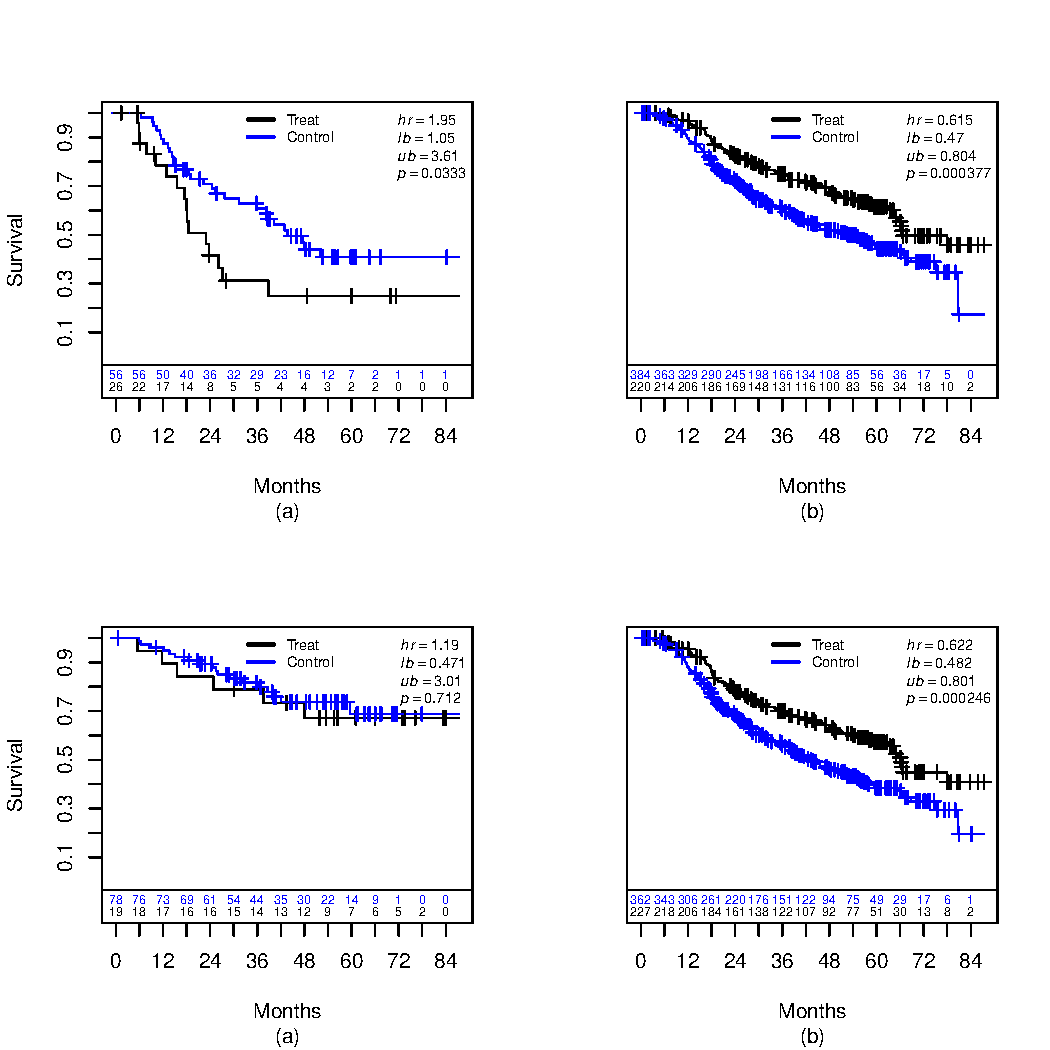
\includegraphics[width=\maxwidth]{figure/unnamed-chunk-2-1} 
\begin{kframe}\begin{alltt}
\hlcom{# plot.subgroup(sub1=check0,sub1C=check1,tte.name='time_months',event.name='status',treat.name='hormon',fix.rows=FALSE,byrisk=6,show.med=FALSE)}
\hlcom{# plot.subgroup(sub1=df0.loh,sub1C=df1.loh,tte.name='time_months',event.name='status',treat.name='hormon',fix.rows=FALSE,byrisk=6,show.med=FALSE)}

\hlkwa{if} \hlstd{(}\hlopt{!}\hlkwd{is.null}\hlstd{(outgrf))} \hlkwd{save}\hlstd{(grf.est,} \hlkwc{file} \hlstd{= outgrf)}
\end{alltt}
\end{kframe}
\end{knitrout}

\begin{knitrout}
\definecolor{shadecolor}{rgb}{0.969, 0.969, 0.969}\color{fgcolor}\begin{kframe}
\begin{alltt}
\hlstd{t.done} \hlkwb{<-} \hlkwd{proc.time}\hlstd{()[}\hlnum{3}\hlstd{]}
\hlstd{t.min} \hlkwb{<-} \hlstd{(t.done} \hlopt{-} \hlstd{t.start.all)}\hlopt{/}\hlnum{60}
\hlkwd{cat}\hlstd{(}\hlstr{"Minutes and hours for GRF estimation"}\hlstd{,} \hlkwd{c}\hlstd{(t.min, t.min}\hlopt{/}\hlnum{60}\hlstd{),} \hlstr{"\textbackslash{}n"}\hlstd{)}
\end{alltt}
\begin{verbatim}
## Minutes and hours for GRF estimation 0.1698667 0.002831111
\end{verbatim}
\end{kframe}
\end{knitrout}


\begin{knitrout}
\definecolor{shadecolor}{rgb}{0.969, 0.969, 0.969}\color{fgcolor}\begin{kframe}
\begin{alltt}
\hlcom{# Recall, GRF splits}

\hlstd{t.start} \hlkwb{<-} \hlkwd{proc.time}\hlstd{()[}\hlnum{3}\hlstd{]}

\hlkwd{cat}\hlstd{(}\hlstr{"GRF variables in selected tree"}\hlstd{,} \hlstr{"\textbackslash{}n"}\hlstd{)}
\end{alltt}
\begin{verbatim}
## GRF variables in selected tree
\end{verbatim}
\begin{alltt}
\hlkwd{print}\hlstd{(grf.est}\hlopt{$}\hlstd{tree.names)}
\end{alltt}
\begin{verbatim}
## [1] "er"
\end{verbatim}
\begin{alltt}
\hlkwd{cat}\hlstd{(}\hlstr{"GRF cuts wrt selected tree:"}\hlstd{,} \hlstr{"\textbackslash{}n"}\hlstd{)}
\end{alltt}
\begin{verbatim}
## GRF cuts wrt selected tree:
\end{verbatim}
\begin{alltt}
\hlkwd{print}\hlstd{(grf.est}\hlopt{$}\hlstd{tree.cuts)}
\end{alltt}
\begin{verbatim}
## [1] "er <= 0"
\end{verbatim}
\begin{alltt}
\hlcom{# Tree 2}
\hlkwd{cat}\hlstd{(}\hlstr{"GRF variables in selected tree 2"}\hlstd{,} \hlstr{"\textbackslash{}n"}\hlstd{)}
\end{alltt}
\begin{verbatim}
## GRF variables in selected tree 2
\end{verbatim}
\begin{alltt}
\hlkwd{print}\hlstd{(grf.est}\hlopt{$}\hlstd{tree2.names)}
\end{alltt}
\begin{verbatim}
## [1] "age" "er"
\end{verbatim}
\begin{alltt}
\hlkwd{cat}\hlstd{(}\hlstr{"GRF cuts wrt selected tree 2:"}\hlstd{,} \hlstr{"\textbackslash{}n"}\hlstd{)}
\end{alltt}
\begin{verbatim}
## GRF cuts wrt selected tree 2:
\end{verbatim}
\begin{alltt}
\hlkwd{print}\hlstd{(grf.est}\hlopt{$}\hlstd{tree2.cuts)}
\end{alltt}
\begin{verbatim}
## [1] "age <= 50" "age <= 43" "er <= 0"
\end{verbatim}
\begin{alltt}
\hlcom{# Tree 3}
\hlkwd{cat}\hlstd{(}\hlstr{"GRF variables in selected tree 3"}\hlstd{,} \hlstr{"\textbackslash{}n"}\hlstd{)}
\end{alltt}
\begin{verbatim}
## GRF variables in selected tree 3
\end{verbatim}
\begin{alltt}
\hlkwd{print}\hlstd{(grf.est}\hlopt{$}\hlstd{tree3.names)}
\end{alltt}
\begin{verbatim}
## [1] "age"  "pgr"  "size" "er"
\end{verbatim}
\begin{alltt}
\hlkwd{cat}\hlstd{(}\hlstr{"GRF cuts wrt selected tree 3:"}\hlstd{,} \hlstr{"\textbackslash{}n"}\hlstd{)}
\end{alltt}
\begin{verbatim}
## GRF cuts wrt selected tree 3:
\end{verbatim}
\begin{alltt}
\hlkwd{print}\hlstd{(grf.est}\hlopt{$}\hlstd{tree3.cuts)}
\end{alltt}
\begin{verbatim}
## [1] "age <= 48"  "pgr <= 8"   "size <= 36" "age <= 33"  "age <= 43" 
## [6] "er <= 0"    "er <= 107"
\end{verbatim}
\begin{alltt}
\hlstd{df.analysis} \hlkwb{<-} \hlstd{gbsg}
\hlstd{df.analysis} \hlkwb{<-} \hlkwd{within}\hlstd{(df.analysis, \{}
    \hlstd{id} \hlkwb{<-} \hlkwd{as.numeric}\hlstd{(}\hlkwd{c}\hlstd{(}\hlnum{1}\hlopt{:}\hlkwd{nrow}\hlstd{(df.analysis)))}
    \hlcom{# time to months}
    \hlstd{time_months} \hlkwb{<-} \hlstd{rfstime}\hlopt{/}\hlnum{30.4375}
    \hlstd{z1a} \hlkwb{<-} \hlkwd{ifelse}\hlstd{(er} \hlopt{<=} \hlnum{0}\hlstd{,} \hlnum{1}\hlstd{,} \hlnum{0}\hlstd{)}
    \hlstd{z1b} \hlkwb{<-} \hlkwd{ifelse}\hlstd{(er} \hlopt{<=} \hlnum{107}\hlstd{,} \hlnum{1}\hlstd{,} \hlnum{0}\hlstd{)}

    \hlstd{z2a} \hlkwb{<-} \hlkwd{ifelse}\hlstd{(pgr} \hlopt{<=} \hlnum{8}\hlstd{,} \hlnum{1}\hlstd{,} \hlnum{0}\hlstd{)}
    \hlstd{z2b} \hlkwb{<-} \hlkwd{ifelse}\hlstd{(pgr} \hlopt{<=} \hlnum{74}\hlstd{,} \hlnum{1}\hlstd{,} \hlnum{0}\hlstd{)}

    \hlstd{z3a} \hlkwb{<-} \hlkwd{ifelse}\hlstd{(age} \hlopt{<=} \hlnum{33}\hlstd{,} \hlnum{1}\hlstd{,} \hlnum{0}\hlstd{)}
    \hlstd{z3b} \hlkwb{<-} \hlkwd{ifelse}\hlstd{(age} \hlopt{<=} \hlnum{43}\hlstd{,} \hlnum{1}\hlstd{,} \hlnum{0}\hlstd{)}
    \hlstd{z3c} \hlkwb{<-} \hlkwd{ifelse}\hlstd{(age} \hlopt{<=} \hlnum{48}\hlstd{,} \hlnum{1}\hlstd{,} \hlnum{0}\hlstd{)}
    \hlstd{z3d} \hlkwb{<-} \hlkwd{ifelse}\hlstd{(age} \hlopt{<=} \hlnum{50}\hlstd{,} \hlnum{1}\hlstd{,} \hlnum{0}\hlstd{)}  \hlcom{# Close to median=53}

    \hlstd{z4} \hlkwb{<-} \hlkwd{ifelse}\hlstd{(meno} \hlopt{==} \hlnum{0}\hlstd{,} \hlnum{1}\hlstd{,} \hlnum{0}\hlstd{)}

    \hlstd{z5} \hlkwb{<-} \hlkwd{ifelse}\hlstd{(nodes} \hlopt{<=} \hlkwd{quantile}\hlstd{(nodes,} \hlkwd{c}\hlstd{(}\hlnum{0.5}\hlstd{)),} \hlnum{1}\hlstd{,} \hlnum{0}\hlstd{)}

    \hlstd{z6} \hlkwb{<-} \hlkwd{ifelse}\hlstd{(size} \hlopt{<=} \hlnum{36}\hlstd{,} \hlnum{1}\hlstd{,} \hlnum{0}\hlstd{)}

    \hlstd{z7a} \hlkwb{<-} \hlkwd{ifelse}\hlstd{(grade} \hlopt{==} \hlnum{1}\hlstd{,} \hlnum{1}\hlstd{,} \hlnum{0}\hlstd{)}
    \hlstd{z7b} \hlkwb{<-} \hlkwd{ifelse}\hlstd{(grade} \hlopt{==} \hlnum{3}\hlstd{,} \hlnum{1}\hlstd{,} \hlnum{0}\hlstd{)}

    \hlcom{# As factors}
    \hlstd{v1a} \hlkwb{<-} \hlkwd{as.factor}\hlstd{(z1a)}
    \hlstd{v1b} \hlkwb{<-} \hlkwd{as.factor}\hlstd{(z1b)}

    \hlstd{v2a} \hlkwb{<-} \hlkwd{as.factor}\hlstd{(z2a)}
    \hlstd{v2b} \hlkwb{<-} \hlkwd{as.factor}\hlstd{(z2b)}

    \hlstd{v3a} \hlkwb{<-} \hlkwd{as.factor}\hlstd{(z3a)}
    \hlstd{v3b} \hlkwb{<-} \hlkwd{as.factor}\hlstd{(z3b)}
    \hlstd{v3c} \hlkwb{<-} \hlkwd{as.factor}\hlstd{(z3c)}
    \hlstd{v3d} \hlkwb{<-} \hlkwd{as.factor}\hlstd{(z3d)}

    \hlstd{v4} \hlkwb{<-} \hlkwd{as.factor}\hlstd{(z4)}
    \hlstd{v5} \hlkwb{<-} \hlkwd{as.factor}\hlstd{(z5)}
    \hlstd{v6} \hlkwb{<-} \hlkwd{as.factor}\hlstd{(z6)}

    \hlstd{v7a} \hlkwb{<-} \hlkwd{as.factor}\hlstd{(z7a)}
    \hlstd{v7b} \hlkwb{<-} \hlkwd{as.factor}\hlstd{(z7b)}
\hlstd{\})}


\hlstd{confounders.name} \hlkwb{<-} \hlkwd{c}\hlstd{(}\hlstr{"v1a"}\hlstd{,} \hlstr{"v1b"}\hlstd{,} \hlstr{"v2a"}\hlstd{,} \hlstr{"v2b"}\hlstd{,} \hlstr{"v3a"}\hlstd{,} \hlstr{"v3b"}\hlstd{,} \hlstr{"v3c"}\hlstd{,} \hlstr{"v3d"}\hlstd{,} \hlstr{"v4"}\hlstd{,}
    \hlstr{"v5"}\hlstd{,} \hlstr{"v6"}\hlstd{,} \hlstr{"v7a"}\hlstd{,} \hlstr{"v7b"}\hlstd{)}

\hlcom{# Note, can try smaller subset to check initial code run}
\hlcom{# confounders.name<-c('v1a','v1b','v1c',}
\hlcom{#'v2a','v2b','v2c',}
\hlcom{#'v3a','v3b','v3c')}

\hlstd{outcome.name} \hlkwb{<-} \hlkwd{c}\hlstd{(}\hlstr{"time_months"}\hlstd{)}
\hlstd{event.name} \hlkwb{<-} \hlkwd{c}\hlstd{(}\hlstr{"status"}\hlstd{)}
\hlstd{id.name} \hlkwb{<-} \hlkwd{c}\hlstd{(}\hlstr{"id"}\hlstd{)}
\hlstd{treat.name} \hlkwb{<-} \hlkwd{c}\hlstd{(}\hlstr{"hormon"}\hlstd{)}

\hlstd{df.confounders} \hlkwb{<-} \hlstd{df.analysis[, confounders.name]}
\hlstd{df.confounders} \hlkwb{<-} \hlkwd{dummy}\hlstd{(df.confounders)}

\hlstd{hr.threshold} \hlkwb{<-} \hlnum{1.5}  \hlcom{# Initital candidates }
\hlstd{hr.consistency} \hlkwb{<-} \hlnum{1.25}  \hlcom{# Candidates for many splits}
\hlstd{pconsistency.threshold} \hlkwb{<-} \hlnum{0.9}
\hlstd{maxk} \hlkwb{<-} \hlnum{4}
\hlcom{# Limit timing for forestsearch}
\hlstd{max.minutes} \hlkwb{<-} \hlnum{60}
\hlstd{nmin.fs} \hlkwb{<-} \hlnum{60}
\hlcom{# stop.threshold<-0.60 # If any sg meets this, then choose this (stop here);}
\hlstd{m1.threshold} \hlkwb{<-} \hlnum{Inf}  \hlcom{# Turning this off (Default)}
\hlstd{stop.threshold} \hlkwb{<-} \hlnum{1}
\hlcom{# =1 will run through all sg's meeting HR criteria}
\hlstd{fs.splits} \hlkwb{<-} \hlnum{1000}  \hlcom{# How many times to split for consistency}
\hlcom{# vi is % factor is selected in cross-validation --> higher more important}
\hlstd{vi.grf.min} \hlkwb{<-} \hlnum{0.2}
\hlcom{# Null, turns off grf screening}

\hlstd{d.min} \hlkwb{<-} \hlnum{10}  \hlcom{# Min number of events for both arms (d0.min=d1.min=d.min)}
\hlcom{# default=5}

\hlstd{sg_focus} \hlkwb{<-} \hlstr{"hr"}


\hlcom{# Default FS implementation (Max consistency with harm) sg_focus<-'Nsg' largest}
\hlcom{# SG with at least pconsistency.threshold}

\hlcom{# The FS algorithm orders subgroups by largest hazard ratios and then cycles}
\hlcom{# through each SG candidate (HR>1.5) to calculate consistency.  Note: there is}
\hlcom{# a pstop_futile input which is default at 0.5, meaning that once a subgroup}
\hlcom{# with consistency less than 50% the algorithm will stop searching: Since}
\hlcom{# meeting 90% consistency for SG's with even lower HR's seems unlikely Setting}
\hlcom{# pstop_futile=0 will cycle through all candidates (HR>1.5)}

\hlstd{fs.est} \hlkwb{<-} \hlkwd{forestsearch}\hlstd{(}\hlkwc{df} \hlstd{= df.analysis,} \hlkwc{confounders.name} \hlstd{= confounders.name,} \hlkwc{df.predict} \hlstd{= df.analysis,}
    \hlkwc{details} \hlstd{=} \hlnum{TRUE}\hlstd{,} \hlkwc{sg_focus} \hlstd{= sg_focus,} \hlkwc{outcome.name} \hlstd{= outcome.name,} \hlkwc{treat.name} \hlstd{= treat.name,}
    \hlkwc{event.name} \hlstd{= event.name,} \hlkwc{id.name} \hlstd{= id.name,} \hlkwc{n.min} \hlstd{= nmin.fs,} \hlkwc{hr.threshold} \hlstd{= hr.threshold,}
    \hlkwc{hr.consistency} \hlstd{= hr.consistency,} \hlkwc{fs.splits} \hlstd{= fs.splits,} \hlkwc{stop.threshold} \hlstd{= stop.threshold,}
    \hlkwc{d0.min} \hlstd{= d.min,} \hlkwc{d1.min} \hlstd{= d.min,} \hlkwc{pconsistency.threshold} \hlstd{= pconsistency.threshold,}
    \hlkwc{max.minutes} \hlstd{= max.minutes,} \hlkwc{maxk} \hlstd{= maxk,} \hlkwc{plot.sg} \hlstd{=} \hlnum{FALSE}\hlstd{,} \hlkwc{vi.grf.min} \hlstd{= vi.grf.min)}
\end{alltt}
\begin{verbatim}
## Confounders per grf screening v1a v2b v1b v5 v7b v3d v2a v6 v3b v4 v3c 
## Number of possible subgroups= 4194303 
## Number of possible subgroups (in millions)= 4.194303 
## # of subgroups based on # variables > k.max and excluded 4185195 
## k.max= 4 
## Events criteria for control,exp= 10 10 
## # of subgroups with events less than criteria: control, experimental 5569 6975 
## # of subgroups meeting all criteria = 1271 
## # of subgroups fitted (Cox model estimable) = 1271 
## Minutes= 0.3021167 
## Number of criteria not met for subgroup evaluation 
## crit.failure
##       0       1       2       3       4 
## 4186466     958    4725     932    1222 
## Number of subgroups meeting HR threshold 65 
## Subgroups (1st 10) meeting overall screening thresholds (HR, m1) sorted by focus: (m1,sg_focus)= Inf hr 
##     K   n  E d1    m1    m0   HR L(HR) U(HR) v1a.0 v1a.1 v2b.0 v2b.1 v1b.0
##  1: 3  78 29 10 17.74   Inf 3.73  1.72  8.08     0     0     0     1     0
##  2: 4  78 29 10 17.74   Inf 3.73  1.72  8.08     0     0     0     1     0
##  3: 4  72 28 10 17.74   Inf 3.58  1.64  7.81     0     0     0     1     0
##  4: 4  77 28 10 17.74   Inf 3.27  1.51  7.11     0     0     0     1     0
##  5: 4  76 26 10 17.74   Inf 2.95  1.33  6.54     1     0     0     1     0
##  6: 3 102 39 13 17.74   Inf 2.90  1.48  5.66     0     0     0     1     0
##  7: 4  85 33 10 27.17   Inf 2.64  1.24  5.62     0     0     0     1     0
##  8: 4  94 37 12 27.17   Inf 2.61  1.31  5.22     0     0     0     1     0
##  9: 2  61 34 15 18.53 47.97 2.54  1.28  5.04     0     1     0     0     0
## 10: 4  85 30 11 37.65   Inf 2.42  1.15  5.10     0     0     0     0     0
##     v1b.1 v5.0 v5.1 v7b.0 v7b.1 v3d.0 v3d.1 v2a.0 v2a.1 v6.0 v6.1 v3b.0 v3b.1
##  1:     0    0    0     0     0     0     0     0     0    0    0     1     0
##  2:     0    0    0     0     0     0     1     0     0    0    0     1     0
##  3:     1    0    0     0     0     0     0     0     0    0    0     1     0
##  4:     0    0    0     0     0     0     1     0     0    0    1     1     0
##  5:     0    0    0     0     0     0     1     0     0    0    0     1     0
##  6:     0    0    0     0     0     0     1     0     0    0    0     1     0
##  7:     0    0    0     0     0     0     1     0     0    0    0     1     0
##  8:     1    0    0     0     0     0     1     0     0    0    0     1     0
##  9:     0    0    0     0     0     0     0     0     0    0    1     0     0
## 10:     1    0    0     0     0     0     0     0     0    0    1     1     0
##     v4.0 v4.1 v3c.0 v3c.1
##  1:    0    0     0     1
##  2:    0    0     0     1
##  3:    0    0     0     1
##  4:    0    0     0     0
##  5:    0    0     0     0
##  6:    0    0     0     0
##  7:    0    1     0     0
##  8:    0    0     0     0
##  9:    0    0     0     0
## 10:    0    0     0     1
## Consistency 0.989 
## Splitting method, # of splits= Random 1000 
## Model, % Consistency Met= v2b.1 v3b.0 v3c.1 0.989 
## Consistency 0.989 
## Splitting method, # of splits= Random 1000 
## Model, % Consistency Met= v2b.1 v3d.1 v3b.0 v3c.1 0.989 
## Consistency 0.988 
## Splitting method, # of splits= Random 1000 
## Model, % Consistency Met= v2b.1 v1b.1 v3b.0 v3c.1 0.988 
## Consistency 0.971 
## Splitting method, # of splits= Random 1000 
## Model, % Consistency Met= v2b.1 v3d.1 v6.1 v3b.0 0.971 
## Consistency 0.952 
## Splitting method, # of splits= Random 1000 
## Model, % Consistency Met= v1a.0 v2b.1 v3d.1 v3b.0 0.952 
## Consistency 0.976 
## Splitting method, # of splits= Random 1000 
## Model, % Consistency Met= v2b.1 v3d.1 v3b.0 0.976 
## Consistency 0.921 
## Splitting method, # of splits= Random 1000 
## Model, % Consistency Met= v2b.1 v3d.1 v3b.0 v4.1 0.921 
## Consistency 0.95 
## Splitting method, # of splits= Random 1000 
## Model, % Consistency Met= v2b.1 v1b.1 v3d.1 v3b.0 0.95 
## Consistency 0.959 
## Splitting method, # of splits= Random 1000 
## Model, % Consistency Met= v1a.1 v6.1 0.959 
## Consistency 0.72 
## Consistency 0.677 
## Consistency 0.554 
## Consistency 0.578 
## Consistency 0.531 
## Consistency 0.619 
## Consistency 0.43 
## Number of subgroups meeting consistency criteria= 9 
##    p.consistency Nsg group.id m.index K   M.1   M.2   M.3   M.4
## 1:         0.989  78       46       1 3 v2b.1 v3b.0 v3c.1      
## 2:         0.989  78       51       2 4 v2b.1 v3d.1 v3b.0 v3c.1
## 3:         0.988  72       47       3 4 v2b.1 v1b.1 v3b.0 v3c.1
## 4:         0.971  77       13       4 4 v2b.1 v3d.1  v6.1 v3b.0
## 5:         0.952  76       23       5 4 v1a.0 v2b.1 v3d.1 v3b.0
## 6:         0.976 102       24       6 3 v2b.1 v3d.1 v3b.0      
## 7:         0.921  85       35       7 4 v2b.1 v3d.1 v3b.0  v4.1
## 8:          0.95  94       25       8 4 v2b.1 v1b.1 v3d.1 v3b.0
## 9:         0.959  61       11       9 2 v1a.1  v6.1            
##    p.consistency Nsg group.id m.index K   M.1   M.2   M.3   M.4
## 1:         0.989  78       46       1 3 v2b.1 v3b.0 v3c.1      
## 2:         0.989  78       51       2 4 v2b.1 v3d.1 v3b.0 v3c.1
## 3:         0.988  72       47       3 4 v2b.1 v1b.1 v3b.0 v3c.1
## 4:         0.976 102       24       6 3 v2b.1 v3d.1 v3b.0      
## 5:         0.971  77       13       4 4 v2b.1 v3d.1  v6.1 v3b.0
## 6:         0.959  61       11       9 2 v1a.1  v6.1            
## 7:         0.952  76       23       5 4 v1a.0 v2b.1 v3d.1 v3b.0
## 8:         0.950  94       25       8 4 v2b.1 v1b.1 v3d.1 v3b.0
## 9:         0.921  85       35       7 4 v2b.1 v3d.1 v3b.0  v4.1
\end{verbatim}
\begin{alltt}
\hlcom{# plot.sg=TRUE will plot the estimated subgroups but this is plotted below}

\hlcom{# These are the frequency each factor appears in a SG combination}

\hlstd{xx} \hlkwb{<-} \hlstd{fs.est}\hlopt{$}\hlstd{find.grps}\hlopt{$}\hlstd{out.found}\hlopt{$}\hlstd{hr.subgroups}
\hlstd{covs.found} \hlkwb{<-} \hlstd{xx[,} \hlopt{-}\hlkwd{c}\hlstd{(}\hlnum{1}\hlopt{:}\hlnum{10}\hlstd{)]}
\hlstd{covs.most} \hlkwb{<-} \hlkwd{apply}\hlstd{(covs.found,} \hlnum{2}\hlstd{, sum)}
\hlstd{covs.most} \hlkwb{<-} \hlstd{covs.most[covs.most} \hlopt{>} \hlnum{0}\hlstd{]}
\hlkwd{print}\hlstd{(covs.most)}
\end{alltt}
\begin{verbatim}
## v1a.0 v1a.1 v2b.1 v1b.1  v5.0 v7b.0 v7b.1 v3d.1 v2a.0 v2a.1  v6.0  v6.1 v3b.0 
##    10     4    28    21     1     7     7    31     1    16     1    10    42 
##  v4.1 v3c.1 
##    13    26
\end{verbatim}
\begin{alltt}
\hlkwd{print}\hlstd{(fs.est}\hlopt{$}\hlstd{grp.consistency}\hlopt{$}\hlstd{result)}
\end{alltt}
\begin{verbatim}
##    p.consistency Nsg group.id m.index K   M.1   M.2   M.3   M.4
## 1:         0.989  78       46       1 3 v2b.1 v3b.0 v3c.1      
## 2:         0.989  78       51       2 4 v2b.1 v3d.1 v3b.0 v3c.1
## 3:         0.988  72       47       3 4 v2b.1 v1b.1 v3b.0 v3c.1
## 4:         0.976 102       24       6 3 v2b.1 v3d.1 v3b.0      
## 5:         0.971  77       13       4 4 v2b.1 v3d.1  v6.1 v3b.0
## 6:         0.959  61       11       9 2 v1a.1  v6.1            
## 7:         0.952  76       23       5 4 v1a.0 v2b.1 v3d.1 v3b.0
## 8:         0.950  94       25       8 4 v2b.1 v1b.1 v3d.1 v3b.0
## 9:         0.921  85       35       7 4 v2b.1 v3d.1 v3b.0  v4.1
\end{verbatim}
\begin{alltt}
\hlstd{df0.fs} \hlkwb{<-} \hlkwd{subset}\hlstd{(fs.est}\hlopt{$}\hlstd{df.pred, treat.recommend} \hlopt{==} \hlnum{0}\hlstd{)}
\hlstd{df1.fs} \hlkwb{<-} \hlkwd{subset}\hlstd{(fs.est}\hlopt{$}\hlstd{df.pred, treat.recommend} \hlopt{==} \hlnum{1}\hlstd{)}

\hlkwa{if} \hlstd{(}\hlopt{!}\hlkwd{is.null}\hlstd{(outfs))} \hlkwd{save}\hlstd{(fs.est, df.analysis, confounders.name,} \hlkwc{file} \hlstd{= outfs)}
\end{alltt}
\end{kframe}
\end{knitrout}



\begin{knitrout}
\definecolor{shadecolor}{rgb}{0.969, 0.969, 0.969}\color{fgcolor}\begin{kframe}
\begin{alltt}
\hlstd{t.done} \hlkwb{<-} \hlkwd{proc.time}\hlstd{()[}\hlnum{3}\hlstd{]}
\hlstd{t.min} \hlkwb{<-} \hlstd{(t.done} \hlopt{-} \hlstd{t.start)}\hlopt{/}\hlnum{60}
\hlkwd{cat}\hlstd{(}\hlstr{"Minutes and hours for FS estimation"}\hlstd{,} \hlkwd{c}\hlstd{(t.min, t.min}\hlopt{/}\hlnum{60}\hlstd{),} \hlstr{"\textbackslash{}n"}\hlstd{)}
\end{alltt}
\begin{verbatim}
## Minutes and hours for FS estimation 0.6980167 0.01163361
\end{verbatim}
\end{kframe}
\end{knitrout}


%\begin{figure}[h!]
%\begin{center}
%<<GBSG_grf-fs_sg,echo=TRUE,out.height="400px",out.width="400px">>=
%# Compare with GRF
%layout(matrix(c(1,2,3,4), 2, 2, byrow = TRUE))
%plot.subgroup(sub1=df0.grf,sub1C=df1.grf,tte.name="time_months",event.name="status",treat.name="hormon",fix.rows=FALSE,byrisk=9,show.med=FALSE,subtitle1="(a)",subtitle2="(b)")
%plot.subgroup(sub1=df0.fs,sub1C=df1.fs,tte.name="time_months",event.name="status",treat.name="hormon",fix.rows=FALSE,byrisk=9,show.med=FALSE,subtitle1="(c)",subtitle2="(d)")
%@
%\end{center}
%\end{figure}


\begin{knitrout}
\definecolor{shadecolor}{rgb}{0.969, 0.969, 0.969}\color{fgcolor}\begin{kframe}
\begin{alltt}
\hlstd{t.start} \hlkwb{<-} \hlkwd{proc.time}\hlstd{()[}\hlnum{3}\hlstd{]}

\hlkwd{library}\hlstd{(doParallel)}
\hlkwd{registerDoParallel}\hlstd{(parallel}\hlopt{::}\hlkwd{detectCores}\hlstd{(}\hlkwc{logical} \hlstd{=} \hlnum{FALSE}\hlstd{))}

\hlstd{cox.formula.boot} \hlkwb{<-} \hlkwd{as.formula}\hlstd{(}\hlkwd{paste}\hlstd{(}\hlstr{"Surv(time_months,status)~hormon"}\hlstd{))}
\hlstd{split_method} \hlkwb{<-} \hlstr{"Random"}
\hlstd{est.loghr} \hlkwb{<-} \hlnum{TRUE}

\hlstd{stop.threshold} \hlkwb{<-} \hlnum{1}
\hlcom{# Can probably set to 0.95 or 0.99, but we set the same as above to mimic the}
\hlcom{# estimation algorithm}
\hlstd{fs.splits} \hlkwb{<-} \hlnum{1000}
\hlstd{max.minutes} \hlkwb{<-} \hlnum{6}

\hlstd{NB} \hlkwb{<-} \hlnum{2000}

\hlstd{df_temp} \hlkwb{<-} \hlstd{fs.est}\hlopt{$}\hlstd{df.pred[,} \hlkwd{c}\hlstd{(}\hlstr{"id"}\hlstd{,} \hlstr{"treat.recommend"}\hlstd{)]}
\hlstd{dfa} \hlkwb{<-} \hlkwd{merge}\hlstd{(df.analysis, df_temp,} \hlkwc{by} \hlstd{=} \hlstr{"id"}\hlstd{)}
\hlstd{df_boot_analysis} \hlkwb{<-} \hlstd{dfa}

\hlstd{fitH} \hlkwb{<-} \hlkwd{get_Cox_sg}\hlstd{(}\hlkwc{df_sg} \hlstd{=} \hlkwd{subset}\hlstd{(df_boot_analysis, treat.recommend} \hlopt{==} \hlnum{0}\hlstd{),} \hlkwc{cox.formula} \hlstd{= cox.formula.boot,}
    \hlkwc{est.loghr} \hlstd{= est.loghr)}
\hlstd{H_obs} \hlkwb{<-} \hlstd{fitH}\hlopt{$}\hlstd{est_obs}  \hlcom{# log(hr) scale}
\hlstd{seH_obs} \hlkwb{<-} \hlstd{fitH}\hlopt{$}\hlstd{se_obs}
\hlcom{# Hc observed estimates}
\hlstd{fitHc} \hlkwb{<-} \hlkwd{get_Cox_sg}\hlstd{(}\hlkwc{df_sg} \hlstd{=} \hlkwd{subset}\hlstd{(df_boot_analysis, treat.recommend} \hlopt{==} \hlnum{1}\hlstd{),} \hlkwc{cox.formula} \hlstd{= cox.formula.boot,}
    \hlkwc{est.loghr} \hlstd{= est.loghr)}
\hlstd{Hc_obs} \hlkwb{<-} \hlstd{fitHc}\hlopt{$}\hlstd{est_obs}
\hlstd{seHc_obs} \hlkwb{<-} \hlstd{fitHc}\hlopt{$}\hlstd{se_obs}
\hlkwd{rm}\hlstd{(}\hlstr{"fitH"}\hlstd{,} \hlstr{"fitHc"}\hlstd{)}

\hlstd{Ystar_mat} \hlkwb{<-} \hlkwd{bootYstar}\hlstd{(\{}
    \hlstd{ystar} \hlkwb{<-} \hlkwd{get_Ystar}\hlstd{(boot)}
\hlstd{\},} \hlkwc{boots} \hlstd{= NB,} \hlkwc{seed} \hlstd{=} \hlnum{8316951}\hlstd{,} \hlkwc{counter} \hlstd{=} \hlstr{"boot"}\hlstd{,} \hlkwc{export} \hlstd{= fun_arg_list_boot)}
\hlcom{# Check dimension}
\hlkwa{if} \hlstd{(}\hlkwd{dim}\hlstd{(Ystar_mat)[}\hlnum{1}\hlstd{]} \hlopt{!=} \hlstd{NB} \hlopt{|} \hlkwd{dim}\hlstd{(Ystar_mat)[}\hlnum{2}\hlstd{]} \hlopt{!=} \hlkwd{nrow}\hlstd{(df_boot_analysis))} \hlkwd{stop}\hlstd{(}\hlstr{"Dimension of Ystar_mat does not match"}\hlstd{)}

\hlstd{tB.start} \hlkwb{<-} \hlkwd{proc.time}\hlstd{()[}\hlnum{3}\hlstd{]}
\hlcom{# Bootstraps}
\hlstd{resB} \hlkwb{<-} \hlkwd{bootPar}\hlstd{(\{}
    \hlstd{ans} \hlkwb{<-} \hlkwd{fsboot_forparallel}\hlstd{(boot)}
\hlstd{\},} \hlkwc{boots} \hlstd{= NB,} \hlkwc{seed} \hlstd{=} \hlnum{8316951}\hlstd{,} \hlkwc{counter} \hlstd{=} \hlstr{"boot"}\hlstd{,} \hlkwc{export} \hlstd{= fun_arg_list_boot)}
\hlstd{tB.now} \hlkwb{<-} \hlkwd{proc.time}\hlstd{()[}\hlnum{3}\hlstd{]}
\hlstd{tB.min} \hlkwb{<-} \hlstd{(tB.now} \hlopt{-} \hlstd{tB.start)}\hlopt{/}\hlnum{60}

\hlstd{doParallel}\hlopt{::}\hlkwd{stopImplicitCluster}\hlstd{()}

\hlkwd{cat}\hlstd{(}\hlstr{"Minutes for Boots"}\hlstd{,} \hlkwd{c}\hlstd{(NB, tB.min),} \hlstr{"\textbackslash{}n"}\hlstd{)}
\end{alltt}
\begin{verbatim}
## Minutes for Boots 2000 116.6073
\end{verbatim}
\begin{alltt}
\hlkwd{cat}\hlstd{(}\hlstr{"Projection per 100"}\hlstd{,} \hlkwd{c}\hlstd{(tB.min} \hlopt{*} \hlstd{(}\hlnum{100}\hlopt{/}\hlstd{NB)),} \hlstr{"\textbackslash{}n"}\hlstd{)}
\end{alltt}
\begin{verbatim}
## Projection per 100 5.830363
\end{verbatim}
\begin{alltt}
\hlkwd{cat}\hlstd{(}\hlstr{"Propn bootstrap subgroups found ="}\hlstd{,} \hlkwd{c}\hlstd{(}\hlkwd{sum}\hlstd{(}\hlopt{!}\hlkwd{is.na}\hlstd{(resB}\hlopt{$}\hlstd{H_biasadj_1))}\hlopt{/}\hlstd{NB),} \hlstr{"\textbackslash{}n"}\hlstd{)}
\end{alltt}
\begin{verbatim}
## Propn bootstrap subgroups found = 0.9515
\end{verbatim}
\begin{alltt}
\hlcom{# How many timmed out}
\hlkwd{cat}\hlstd{(}\hlstr{"Number timmed out="}\hlstd{,} \hlkwd{c}\hlstd{(}\hlkwd{sum}\hlstd{(}\hlkwd{is.na}\hlstd{(resB}\hlopt{$}\hlstd{H_biasadj_1)} \hlopt{&} \hlstd{resB}\hlopt{$}\hlstd{tmins_search} \hlopt{>} \hlstd{max.minutes)),}
    \hlstr{"\textbackslash{}n"}\hlstd{)}
\end{alltt}
\begin{verbatim}
## Number timmed out= 0
\end{verbatim}
\begin{alltt}
\hlstd{H_estimates} \hlkwb{<-} \hlkwd{get_dfRes}\hlstd{(}\hlkwc{Hobs} \hlstd{= H_obs,} \hlkwc{seHobs} \hlstd{= seH_obs,} \hlkwc{H1_adj} \hlstd{= resB}\hlopt{$}\hlstd{H_biasadj_1,}
    \hlkwc{ystar} \hlstd{= Ystar_mat,} \hlkwc{cov_method} \hlstd{=} \hlstr{"standard"}\hlstd{,} \hlkwc{cov_trim} \hlstd{=} \hlnum{0.05}\hlstd{)}

\hlstd{Hc_estimates} \hlkwb{<-} \hlkwd{get_dfRes}\hlstd{(}\hlkwc{Hobs} \hlstd{= Hc_obs,} \hlkwc{seHobs} \hlstd{= seHc_obs,} \hlkwc{H1_adj} \hlstd{= resB}\hlopt{$}\hlstd{Hc_biasadj_1,}
    \hlkwc{ystar} \hlstd{= Ystar_mat,} \hlkwc{cov_method} \hlstd{=} \hlstr{"standard"}\hlstd{,} \hlkwc{cov_trim} \hlstd{=} \hlnum{0.05}\hlstd{)}

\hlkwd{print}\hlstd{(H_estimates)}
\end{alltt}
\begin{verbatim}
##          H0     sdH0 H0_lower H0_upper       H1      sdH1 H1_lower H1_upper
## 1: 3.729046 1.470716 1.721426 8.078059 2.260805 0.4491633 1.531621 3.337142
\end{verbatim}
\begin{alltt}
\hlkwd{print}\hlstd{(Hc_estimates)}
\end{alltt}
\begin{verbatim}
##           H0       sdH0  H0_lower  H0_upper        H1       sdH1  H1_lower
## 1: 0.5950175 0.07852577 0.4594041 0.7706634 0.6295678 0.08331257 0.4857362
##     H1_upper
## 1: 0.8159894
\end{verbatim}
\begin{alltt}
\hlkwa{if} \hlstd{(}\hlopt{!}\hlkwd{is.null}\hlstd{(outfsboot))} \hlkwd{save}\hlstd{(fs.est, Ystar_mat, resB, H_estimates, Hc_estimates,}
    \hlstd{df_boot_analysis,} \hlkwc{file} \hlstd{= outfsboot)}
\end{alltt}
\end{kframe}
\end{knitrout}



\begin{knitrout}
\definecolor{shadecolor}{rgb}{0.969, 0.969, 0.969}\color{fgcolor}\begin{kframe}
\begin{alltt}
\hlstd{t.done} \hlkwb{<-} \hlkwd{proc.time}\hlstd{()[}\hlnum{3}\hlstd{]}
\hlstd{t.min} \hlkwb{<-} \hlstd{(t.done} \hlopt{-} \hlstd{t.start)}\hlopt{/}\hlnum{60}
\hlkwd{cat}\hlstd{(}\hlstr{"Minutes and hours for FS bootstrap"}\hlstd{,} \hlkwd{c}\hlstd{(t.min, t.min}\hlopt{/}\hlnum{60}\hlstd{),} \hlstr{"\textbackslash{}n"}\hlstd{)}
\end{alltt}
\begin{verbatim}
## Minutes and hours for FS bootstrap 116.6216 1.943693
\end{verbatim}
\end{kframe}
\end{knitrout}



\begin{knitrout}
\definecolor{shadecolor}{rgb}{0.969, 0.969, 0.969}\color{fgcolor}\begin{kframe}
\begin{alltt}
\hlstd{df0.fs} \hlkwb{<-} \hlkwd{subset}\hlstd{(fs.est}\hlopt{$}\hlstd{df.pred, treat.recommend} \hlopt{==} \hlnum{0}\hlstd{)}
\hlstd{df1.fs} \hlkwb{<-} \hlkwd{subset}\hlstd{(fs.est}\hlopt{$}\hlstd{df.pred, treat.recommend} \hlopt{==} \hlnum{1}\hlstd{)}

\hlcom{# ITT analysis}
\hlstd{cox_itt} \hlkwb{<-} \hlkwd{summary}\hlstd{(}\hlkwd{coxph}\hlstd{(}\hlkwd{Surv}\hlstd{(time_months, status)} \hlopt{~} \hlstd{hormon,} \hlkwc{data} \hlstd{= fs.est}\hlopt{$}\hlstd{df.pred))}\hlopt{$}\hlstd{conf.int}

\hlcom{# ITT estimates}
\hlstd{resITT} \hlkwb{<-} \hlkwd{c}\hlstd{(}\hlkwd{round}\hlstd{(cox_itt[}\hlkwd{c}\hlstd{(}\hlnum{1}\hlstd{,} \hlnum{3}\hlstd{,} \hlnum{4}\hlstd{)],} \hlnum{2}\hlstd{),} \hlkwd{nrow}\hlstd{(fs.est}\hlopt{$}\hlstd{df.pred))}

\hlcom{# Forest Search Un-adjusted}
\hlstd{Hstat} \hlkwb{<-} \hlkwd{c}\hlstd{(}\hlkwd{unlist}\hlstd{(H_estimates))[}\hlkwd{c}\hlstd{(}\hlnum{1}\hlstd{,} \hlnum{3}\hlstd{,} \hlnum{4}\hlstd{)]}
\hlstd{resH_obs} \hlkwb{<-} \hlkwd{c}\hlstd{(}\hlkwd{c}\hlstd{(Hstat),} \hlkwd{nrow}\hlstd{(df0.fs))}
\hlcom{# Bias-corrected}
\hlstd{Hstat} \hlkwb{<-} \hlkwd{c}\hlstd{(}\hlkwd{unlist}\hlstd{(H_estimates))[}\hlkwd{c}\hlstd{(}\hlnum{5}\hlstd{,} \hlnum{7}\hlstd{,} \hlnum{8}\hlstd{)]}
\hlstd{resH_bc} \hlkwb{<-} \hlkwd{c}\hlstd{(}\hlkwd{c}\hlstd{(Hstat),} \hlkwd{nrow}\hlstd{(df0.fs))}

\hlstd{Hstat2} \hlkwb{<-} \hlkwd{c}\hlstd{(}\hlkwd{unlist}\hlstd{(H_estimates))[}\hlkwd{c}\hlstd{(}\hlnum{5}\hlstd{,} \hlnum{7}\hlstd{,} \hlnum{8}\hlstd{)]}
\hlstd{Hstat2} \hlkwb{<-} \hlkwd{round}\hlstd{(Hstat2,} \hlnum{2}\hlstd{)}
\hlstd{a} \hlkwb{<-} \hlkwd{paste0}\hlstd{(Hstat2[}\hlnum{1}\hlstd{],} \hlstr{" ["}\hlstd{)}
\hlstd{a} \hlkwb{<-} \hlkwd{paste0}\hlstd{(a, Hstat2[}\hlnum{2}\hlstd{])}
\hlstd{a} \hlkwb{<-} \hlkwd{paste0}\hlstd{(a,} \hlstr{","}\hlstd{)}
\hlstd{a} \hlkwb{<-} \hlkwd{paste0}\hlstd{(a, Hstat2[}\hlnum{3}\hlstd{])}
\hlstd{a} \hlkwb{<-} \hlkwd{paste0}\hlstd{(a,} \hlstr{"]"}\hlstd{)}
\hlstd{H_bc2} \hlkwb{<-} \hlkwd{c}\hlstd{(a)}

\hlcom{# Un-adjusted}
\hlstd{Hcstat} \hlkwb{<-} \hlkwd{c}\hlstd{(}\hlkwd{unlist}\hlstd{(Hc_estimates))[}\hlkwd{c}\hlstd{(}\hlnum{1}\hlstd{,} \hlnum{3}\hlstd{,} \hlnum{4}\hlstd{)]}
\hlstd{resHc_obs} \hlkwb{<-} \hlkwd{c}\hlstd{(}\hlkwd{c}\hlstd{(Hcstat),} \hlkwd{nrow}\hlstd{(df1.fs))}
\hlcom{# Bias-corrected}
\hlstd{Hcstat} \hlkwb{<-} \hlkwd{c}\hlstd{(}\hlkwd{unlist}\hlstd{(Hc_estimates))[}\hlkwd{c}\hlstd{(}\hlnum{5}\hlstd{,} \hlnum{7}\hlstd{,} \hlnum{8}\hlstd{)]}
\hlstd{resHc_bc} \hlkwb{<-} \hlkwd{c}\hlstd{(}\hlkwd{c}\hlstd{(Hcstat),} \hlkwd{nrow}\hlstd{(df1.fs))}


\hlstd{Hcstat2} \hlkwb{<-} \hlkwd{c}\hlstd{(}\hlkwd{unlist}\hlstd{(Hc_estimates))[}\hlkwd{c}\hlstd{(}\hlnum{5}\hlstd{,} \hlnum{7}\hlstd{,} \hlnum{8}\hlstd{)]}
\hlstd{Hcstat2} \hlkwb{<-} \hlkwd{round}\hlstd{(Hcstat2,} \hlnum{2}\hlstd{)}
\hlstd{a} \hlkwb{<-} \hlkwd{paste0}\hlstd{(Hcstat2[}\hlnum{1}\hlstd{],} \hlstr{" ["}\hlstd{)}
\hlstd{a} \hlkwb{<-} \hlkwd{paste0}\hlstd{(a, Hcstat2[}\hlnum{2}\hlstd{])}
\hlstd{a} \hlkwb{<-} \hlkwd{paste0}\hlstd{(a,} \hlstr{","}\hlstd{)}
\hlstd{a} \hlkwb{<-} \hlkwd{paste0}\hlstd{(a, Hcstat2[}\hlnum{3}\hlstd{])}
\hlstd{a} \hlkwb{<-} \hlkwd{paste0}\hlstd{(a,} \hlstr{"]"}\hlstd{)}
\hlstd{Hc_bc2} \hlkwb{<-} \hlkwd{c}\hlstd{(a)}

\hlstd{res} \hlkwb{<-} \hlkwd{rbind}\hlstd{(resITT, resH_obs, resH_bc, resHc_obs, resHc_bc)}

\hlstd{resf} \hlkwb{<-} \hlkwd{as.data.frame}\hlstd{(res)}

\hlkwd{colnames}\hlstd{(resf)} \hlkwb{<-} \hlkwd{c}\hlstd{(}\hlstr{"HR Estimate"}\hlstd{,} \hlstr{"Lower"}\hlstd{,} \hlstr{"Upper"}\hlstd{,} \hlstr{"$\textbackslash{}\textbackslash{}#$ Subjects"}\hlstd{)}

\hlstd{rnH} \hlkwb{<-} \hlkwd{c}\hlstd{(}\hlstr{"$\textbackslash{}\textbackslash{}hat\{H\}$"}\hlstd{,} \hlstr{"$\textbackslash{}\textbackslash{}hat\{H\}_\{bc\}$"}\hlstd{)}
\hlstd{rnHc} \hlkwb{<-} \hlkwd{c}\hlstd{(}\hlstr{"$\textbackslash{}\textbackslash{}hat\{H\}^\{c\}$"}\hlstd{,} \hlstr{"$\textbackslash{}\textbackslash{}hat\{H\}^\{c\}_\{bc\}$"}\hlstd{)}
\hlstd{rnItt} \hlkwb{<-} \hlkwd{c}\hlstd{(}\hlstr{"ITT"}\hlstd{)}
\hlkwd{rownames}\hlstd{(resf)} \hlkwb{<-} \hlkwd{c}\hlstd{(rnItt, rnH, rnHc)}
\end{alltt}
\end{kframe}
\end{knitrout}


\begin{knitrout}
\definecolor{shadecolor}{rgb}{0.969, 0.969, 0.969}\color{fgcolor}\begin{kframe}
\begin{alltt}
\hlcom{# Resolve conflict with dplyr}
\hlkwd{library}\hlstd{(conflicted)}
\hlstd{group_rows} \hlkwb{<-} \hlstd{kableExtra}\hlopt{::}\hlstd{group_rows}

\hlkwd{options}\hlstd{(}\hlkwc{knitr.kable.NA} \hlstd{=} \hlstr{"."}\hlstd{,} \hlkwc{format} \hlstd{=} \hlstr{"latex"}\hlstd{)}
\hlstd{tab_gbsg} \hlkwb{<-} \hlkwd{kbl}\hlstd{(resf,} \hlkwc{longtable} \hlstd{=} \hlnum{FALSE}\hlstd{,} \hlkwc{align} \hlstd{=} \hlstr{"c"}\hlstd{,} \hlkwc{format} \hlstd{=} \hlstr{"latex"}\hlstd{,} \hlkwc{booktabs} \hlstd{=} \hlnum{TRUE}\hlstd{,}
    \hlkwc{escape} \hlstd{= F,} \hlkwc{digits} \hlstd{=} \hlnum{3}\hlstd{,} \hlkwc{caption} \hlstd{=} \hlstr{"\textbackslash{}\textbackslash{}label\{tab:gbsg\} GBSG FS Analysis: Cox hazard ratio (HR) estimates for the ITT population and subgroups $H$ and $H^\{c\}$.
Cox model estimates are based on subgroups: The estimated subgroup $\textbackslash{}\textbackslash{}hat\{H\}$; and 
the bootstrap ($B=2000$) bias-correction to $\textbackslash{}\textbackslash{}hat\{H\}$ estimates, denoted $\textbackslash{}\textbackslash{}hat\{H\}_\{bc\}$.  Estimates for the complement $H^\{c\}$ are defined analogously.
The number of subjects in each population ($\textbackslash{}\textbackslash{}#$ Subjects) are listed."}\hlstd{)} \hlopt
    \hlkwd{kable_styling}\hlstd{(}\hlkwc{full_width} \hlstd{=} \hlnum{FALSE}\hlstd{,} \hlkwc{font_size} \hlstd{=} \hlnum{9}\hlstd{,} \hlkwc{latex_options} \hlstd{=} \hlstr{"hold_position"}\hlstd{)} \hlopt
    \hlkwd{group_rows}\hlstd{(}\hlstr{"ITT"}\hlstd{,} \hlnum{1}\hlstd{,} \hlnum{1}\hlstd{)} \hlopt
    \hlkwd{group_rows}\hlstd{(}\hlstr{"H subgroup estimates"}\hlstd{,} \hlnum{2}\hlstd{,} \hlnum{3}\hlstd{)} \hlopt
    \hlkwd{group_rows}\hlstd{(}\hlstr{"H-complement subgroup estimates"}\hlstd{,} \hlnum{4}\hlstd{,} \hlnum{5}\hlstd{)}
\end{alltt}
\end{kframe}
\end{knitrout}

\begin{table}[!h]

\caption{\label{tab:fs_tab}\label{tab:gbsg} GBSG FS Analysis: Cox hazard ratio (HR) estimates for the ITT population and subgroups $H$ and $H^{c}$.
Cox model estimates are based on subgroups: The estimated subgroup $\hat{H}$; and 
the bootstrap ($B=2000$) bias-correction to $\hat{H}$ estimates, denoted $\hat{H}_{bc}$.  Estimates for the complement $H^{c}$ are defined analogously.
The number of subjects in each population ($\#$ Subjects) are listed.}
\centering
\fontsize{9}{11}\selectfont
\begin{tabular}[t]{lcccc}
\toprule
  & HR Estimate & Lower & Upper & $\#$ Subjects\\
\midrule
\addlinespace[0.3em]
\multicolumn{5}{l}{\textbf{ITT}}\\
\hspace{1em}ITT & 0.690 & 0.540 & 0.890 & 686\\
\addlinespace[0.3em]
\multicolumn{5}{l}{\textbf{H subgroup estimates}}\\
\hspace{1em}$\hat{H}$ & 3.729 & 1.721 & 8.078 & 78\\
\hspace{1em}$\hat{H}_{bc}$ & 2.261 & 1.532 & 3.337 & 78\\
\addlinespace[0.3em]
\multicolumn{5}{l}{\textbf{H-complement subgroup estimates}}\\
\hspace{1em}$\hat{H}^{c}$ & 0.595 & 0.459 & 0.771 & 608\\
\hspace{1em}$\hat{H}^{c}_{bc}$ & 0.630 & 0.486 & 0.816 & 608\\
\bottomrule
\end{tabular}
\end{table}



\begin{knitrout}
\definecolor{shadecolor}{rgb}{0.969, 0.969, 0.969}\color{fgcolor}\begin{kframe}
\begin{alltt}
\hlstd{t.done} \hlkwb{<-} \hlkwd{proc.time}\hlstd{()[}\hlnum{3}\hlstd{]}
\hlstd{t.min} \hlkwb{<-} \hlstd{(t.done} \hlopt{-} \hlstd{t.start.all)}\hlopt{/}\hlnum{60}
\hlkwd{cat}\hlstd{(}\hlstr{"Minutes and hours to finish"}\hlstd{,} \hlkwd{c}\hlstd{(t.min, t.min}\hlopt{/}\hlnum{60}\hlstd{),} \hlstr{"\textbackslash{}n"}\hlstd{)}
\end{alltt}
\begin{verbatim}
## Minutes and hours to finish 117.4924 1.958207
\end{verbatim}
\begin{alltt}
\hlkwd{cat}\hlstd{(}\hlstr{"Machine="}\hlstd{,} \hlkwd{c}\hlstd{(}\hlkwd{Sys.info}\hlstd{()[[}\hlnum{4}\hlstd{]]),} \hlstr{"\textbackslash{}n"}\hlstd{)}
\end{alltt}
\begin{verbatim}
## Machine= Mac-Studio-M1-Ultra-2022.local
\end{verbatim}
\begin{alltt}
\hlkwd{cat}\hlstd{(}\hlstr{"Number of cores="}\hlstd{,} \hlkwd{c}\hlstd{(}\hlkwd{detectCores}\hlstd{(}\hlkwc{logical} \hlstd{=} \hlnum{FALSE}\hlstd{)),} \hlstr{"\textbackslash{}n"}\hlstd{)}
\end{alltt}
\begin{verbatim}
## Number of cores= 20
\end{verbatim}
\end{kframe}
\end{knitrout}


\end{document}

@
